\begin{figure}
\begin{center}

% 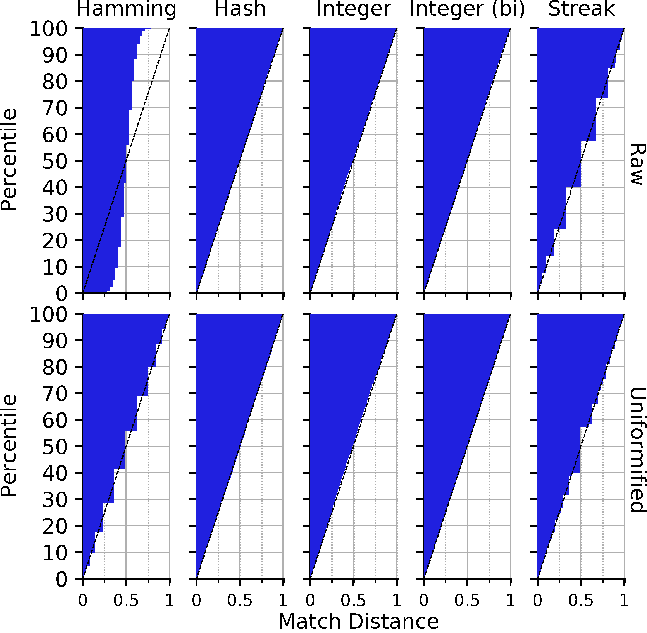
\includegraphics[width=\columnwidth]{img/uniformification/bitweight=0dot5+seed=1+title=low-score-distribution+_data_hathash_hash=75684cf1e73fb7f1+_script_fullcat_hash=c3113c80efb02374+ext=}
\begin{minipage}{\linewidth}
\begin{subfigure}[b]{\linewidth}
\begin{minipage}{0.75\textwidth}
\begin{center}
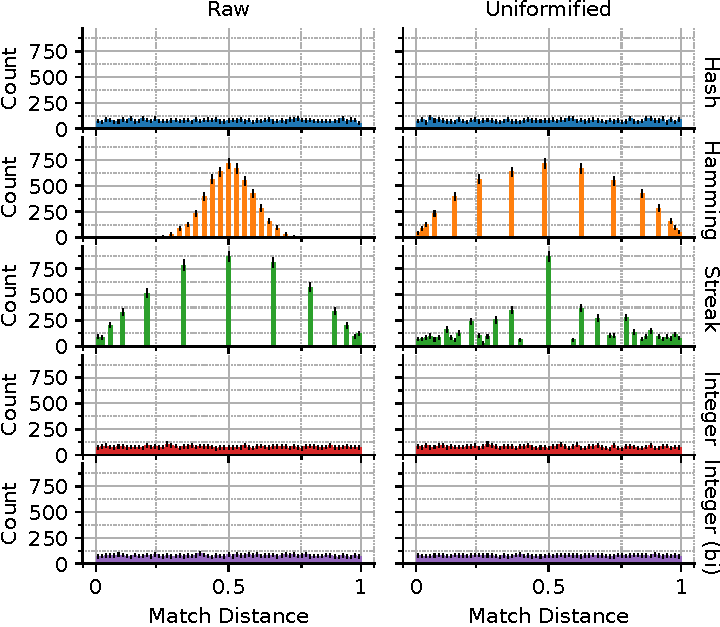
\includegraphics[width=\columnwidth]{img/uniformification/bitweight=0dot5+seed=1+title=low-score-distribution+viz=hist+_data_hathash_hash=75684cf1e73fb7f1+_script_fullcat_hash=dc969d47b9aa144d+ext=}
\end{center}
\end{minipage}
\begin{minipage}{0.23\textwidth}
\caption{
Histogram visualization of match distance between randomly sampled tags.
The bin count of 65 was chosen to emphasize the coarse match distance discretization imposed by the Streak metric and the Hamming metric.\footnotemark
Error bars are 95\% confidence intervals calculated using the Wilson score method with continuity correction \citep{newcombe1998two}.
}
\label{fig:uniformification_hist}
\end{minipage}
\end{subfigure}
\end{minipage}

\begin{minipage}{\linewidth}
\begin{subfigure}[b]{\linewidth}
\begin{minipage}{0.75\textwidth}
\begin{center}
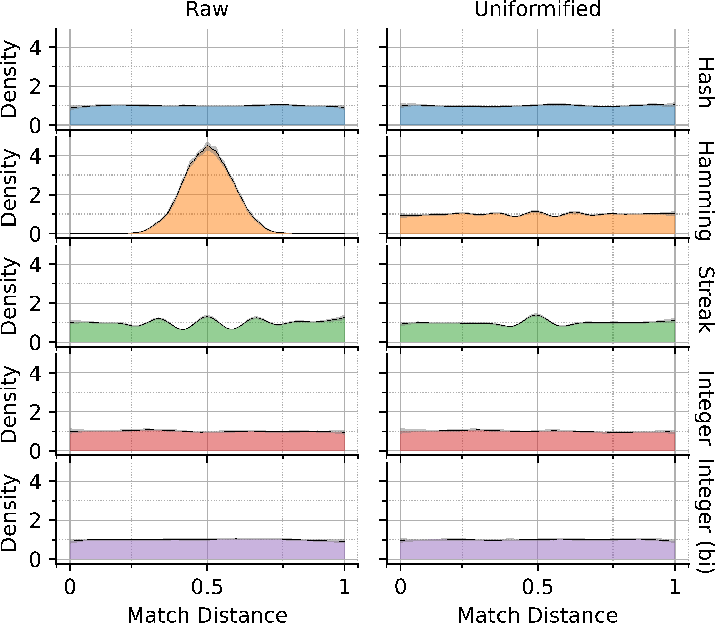
\includegraphics[width=\columnwidth]{img/uniformification/bitweight=0dot5+seed=1+title=low-score-distribution+viz=kde+_data_hathash_hash=75684cf1e73fb7f1+_script_fullcat_hash=73c1663bd9b49595+ext=}
\end{center}
\end{minipage}
\begin{minipage}{0.23\textwidth}
\caption{
Kernel density estimate visualization of match distance between randomly sampled tags.
Estimated density incorporates linear combination correction for bounded distributions due to restriction of match distance within the interval $[0,1]$ \citep{jones1993simple}.
Gray error bands are bootstrap 95\% confidence intervals over 1,000 resamplings.
}
\label{fig:uniformification_kde}
\end{minipage}
\end{subfigure}
\end{minipage}

\caption{
Distance distributions of metrics before and after uniformification.
A sample of 5,000 distances between randomly-generated tag pairs was used for each plot.
Subfigure \ref{fig:uniformification_hist} emphasizes the discretization artifacts in the Hamming and Streak metrics present before and remaining after uniformification.
(E.g., for 32-bit tags under the Hamming metric only 33 distinguishable match distance values are possible.)
Subfigure \ref{fig:uniformification_kde} masks distribution discretization to more intuitively depict the corrected metrics' approximation of a uniform distribution.
Supplementary Figure \ref{fig:uniformification_supp} visualizes the cumulative distribution of all 5,000 sampled distances for each metric before and after uniformification.
}
\label{fig:uniformification}

\end{center}
\end{figure}

\footnotetext{
The uniformified score for the Hamming metric's median matching case falls into the slightly leftern 31st bin instead of the central 32nd bin.
This true median value for the Hamming metric was approximated to a match distance of 0.4901.
This outcome falls within the outer extreme, but still plausible, error of the Monte Carlo approximation, at $p=0.024$ under a double-tailed exact binomial test.
Given the five uniformifications performed (one for each metric), this result is less surprising still.
See main text for detailed discussion of expected error under the Monte Carlo approximation method.
}
